\begin{figure}[t]
\centering
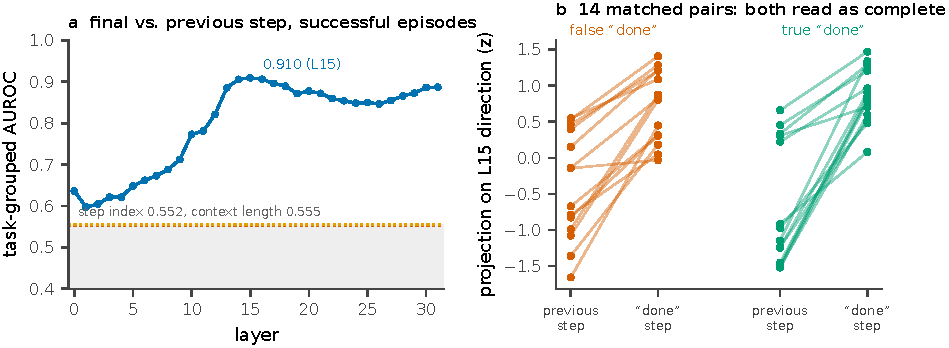
\includegraphics[width=\linewidth]{figs/perceive.pdf}
\caption{\textbf{An imminent-completion direction beats position but does not separate false from true completions.} Exploratory, no causal test. (a)~Task-grouped AUROC of a direction learned inside successful episodes (final \texttt{answer} step vs.\ the step before it, \pcPairs{} pairs, \pcTasks{} tasks), by layer; the grey band is at or below the position baselines. (b)~Cross-fitted projections at layer \pcLayer{} on \pcMatchN{} matched pairs: the projection rises at the ``done'' step for false and true completions alike.}
\label{fig:perceive}
\end{figure}
